\documentclass[presentation]{beamer}

\usepackage{tikz}
\usetikzlibrary{positioning,calc}
\usetikzlibrary{shapes.geometric}
\usetikzlibrary{backgrounds}% only to show the bounding box
\usetikzlibrary{shapes,arrows}
\usepackage{pgfplots}
\usepackage{pgfplotstable}
\usetikzlibrary{pgfplots.groupplots}
\pgfplotsset{compat=1.12}
\usepackage{appendixnumberbeamer}
\usepackage{amsmath}
\date{8th June 2016}
\usetheme{metropolis}

\pgfplotscreateplotcyclelist{decent cycle}{%
  {blue, mark=*, mark options={fill=blue},
    mark size=2pt},
  {cyan, mark=square*, mark options={fill=cyan},
    mark size=2pt},
  {magenta, mark=triangle*, mark options={fill=magenta},
    mark size=3pt},
  {blue, mark=*, mark options={fill=blue},
    mark size=2pt},
  {cyan, mark=square*, mark options={fill=cyan},
    mark size=2pt},
  {magenta, mark=triangle*, mark options={fill=magenta},
    mark size=3pt},
}

\pgfplotsset{
  decent/.style={
    cycle list name=decent cycle,
  }
}
\renewcommand{\vec}[1]{\ensuremath{\boldsymbol{#1}}}
\newcommand{\ddt}[1]{\frac{\partial #1}{\partial t}}
\newcommand{\zhat}{\hat{\vec{z}}}
\newcommand{\W}{\ensuremath{\mathbb{W}}}

\DeclareMathOperator{\grad}{grad}
\let\div\relax
\DeclareMathOperator{\div}{div}
\DeclareMathOperator{\curl}{curl}
\newcommand{\vsubset}[1]{\rotatebox[origin=c]{90}{\ensuremath{\subset}}}
\newcommand{\inner}[2]{\ensuremath{\langle #1, #2 \rangle}}
\author{Lawrence Mitchell\inst{1}}
\institute{
\inst{1}Departments of Computing and Mathematics, Imperial College
London
}

\graphicspath{{./\jobname.figures/}}

\newcommand{\arxivlink}[2]{%
  \href{http://www.arxiv.org/abs/#1}%
  {{\small\texttt{arXiv:\,#1\,[#2]}}}%
}
\newcommand{\doilink}[1]{%
  \href{http://dx.doi.org/#1}%
  {{\small\texttt{doi:\,#1}{}}}%
}
\usepackage[url=false,
            doi=true,
            isbn=false,
            style=authoryear,
            firstinits=true,
            uniquename=init,
            backend=biber]{biblatex}

\setbeamertemplate{bibliography item}{}
\renewcommand{\bibfont}{\scriptsize}
\addbibresource{references.bib}

\setlength{\bibitemsep}{1ex}

\renewbibmacro{in:}{}
\DeclareFieldFormat[article]{volume}{\textbf{#1}}
\DeclareFieldFormat{doi}{%
  doi\addcolon%
  {\scriptsize\ifhyperref{\href{http://dx.doi.org/#1}{\nolinkurl{#1}}}
    {\nolinkurl{#1}}}}
\AtEveryBibitem{%
\clearfield{pages}%
\clearfield{issue}%
\clearfield{number}%
}

\usepackage{minted}

\title{Firedrake: automating the finite element method by composing
  abstractions}

\begin{document}
\maketitle

\begin{frame}
  \frametitle{Firedrake development team}
  \begin{itemize}
  \item[IC] David A.~Ham, Mikl\'os Homolya, Fabio Luporini, Gheorghe-Teodor
    Bercea, Paul H.~J.~Kelly
  \item[Bath] Andrew T.~T.~McRae
  \item[ECMWF] Florian Rathgeber
  \end{itemize}
  \begin{center}
    \uncover<2->{\url{www.firedrakeproject.org}}\\
    \uncover<3->{\cite{Rathgeber:2015} \arxivlink{1501.01809}{cs.MS}}
  \end{center}
\end{frame}

\section{The right abstraction level}

\begin{frame}[fragile]
  \frametitle{How do \emph{you} solve the Poisson equation?}
  \begin{columns}
    \begin{column}{0.65\textwidth}
\begin{minted}[fontsize=\tiny]{python}
from firedrake import *
mesh = UnitSquareMesh(100, 100)
V = FunctionSpace(mesh, "RT", 2)
Q = FunctionSpace(mesh, "DG", 1)
W = V*Q
u, p = TrialFunctions(W)
v, q = TestFunctions(W)

a = dot(u, v)*dx + div(v)*p*dx + div(u)*q*dx
L = -Constant(1)*v*dx
u = Function(W)
solve(a == L, u, solver_parameters={
    "ksp_type": "gmres", 
    "ksp_rtol": 1e-8,
    "pc_type": "fieldsplit",
    "pc_fieldsplit_type": "schur",
    "pc_fieldsplit_schur_fact_type": "full",
    "pc_fieldsplit_schur_precondition": "selfp",
    "fieldsplit_0_ksp_type": "preonly",
    "fieldsplit_0_pc_type": "ilu",
    "fieldsplit_1_ksp_type": "preonly",
    "fieldsplit_1_pc_type": "hypre"
})
\end{minted}
    \end{column}
    \hspace{-4em}
    \begin{column}{0.5\textwidth}
      Find $u\in V\times Q\subset H(\div)\times L^2$ s.t.
      \begin{align*}
        \inner{u}{v} + \inner{\div v}{p} &= 0 \quad\forall\, v \in V\\
        \inner{\div u}{q} &= -\inner{1}{q}\quad\forall\, q \in Q.
      \end{align*}
    \end{column}
  \end{columns}
\end{frame}


\begin{frame}
  \frametitle{Developing models}

  \begin{itemize}
  \item Choose equations
  \item Pick method/discretisation
  \item Decide on implementation language, target architecture
  \item Write code
  \item ...
  \item Optimise
  \item ...
  \item Profit?
  \end{itemize}
\end{frame}

\begin{frame}
  \frametitle{Experimentation should be easy}
  How much code do you need to change to
  \begin{itemize}
  \item Change preconditioner (e.g.~ILU to AMG)?
  \item Drop terms in the preconditioning operator?
  \item Use a completely different operator to precondition?
  \item Do quasi-Newton with an approximate Jacobian?
  \item Apply operators matrix-free?
  \end{itemize}
\end{frame}


\begin{frame}[standout]
  \only<1>{Can we offer easy experimentation without compromising performance?}
  \only<2>{Can we offer easy experimentation without compromising
    performance \emph{too much}?}
\end{frame}


\begin{frame}[fragile]
  \frametitle{FEM pseudocode}
  \begin{onlyenv}<1>
\begin{minted}[fontsize=\tiny]{python}
# x the input fields (e.g. current guess)
def form_residual(x):
    x_l <- x # global to ghosted
    for each element in mesh:
        x_e <- x_l[element] # gather through element map
        for each qp in element:
            basis_fns <- eval_basis_funs(qp)
            J <- compute_geometry(element, qp)
            for each bf in basis_fns:
                x_e_qp <- eval(x_e at qp)
                f_qp <- user_evaluation(qp, bf, x_e_qp)
            # insert into element residual
            f_e <- transform_to_physical(f_qp, J)
        f_l <- f_e # scatter through element map
    f <- f_l # ghosted to global
\end{minted}
  \end{onlyenv}

  \begin{onlyenv}<2>
\begin{minted}[fontsize=\tiny]{python}
                f_qp <- user_evaluation(qp, bf, x_e_qp)
\end{minted}
    \begin{itemize}
    \item Problem-specific variability in \emph{innermost} loop
    \item Efficient implementation may need to:
      \begin{itemize}
      \item vectorize across elements,
      \item vectorize within an element,
      \item exchange loop orders,
      \item hoist loop-invariant code,
      \item exploit structure in basis functions,
      \item pre-evaluate geometry at quad points.
      \item ...
      \end{itemize}
    \end{itemize}
  \end{onlyenv}
\end{frame}

\begin{frame}[standout]
  Say \emph{what}, not \emph{how}.
\end{frame}

\begin{frame}
  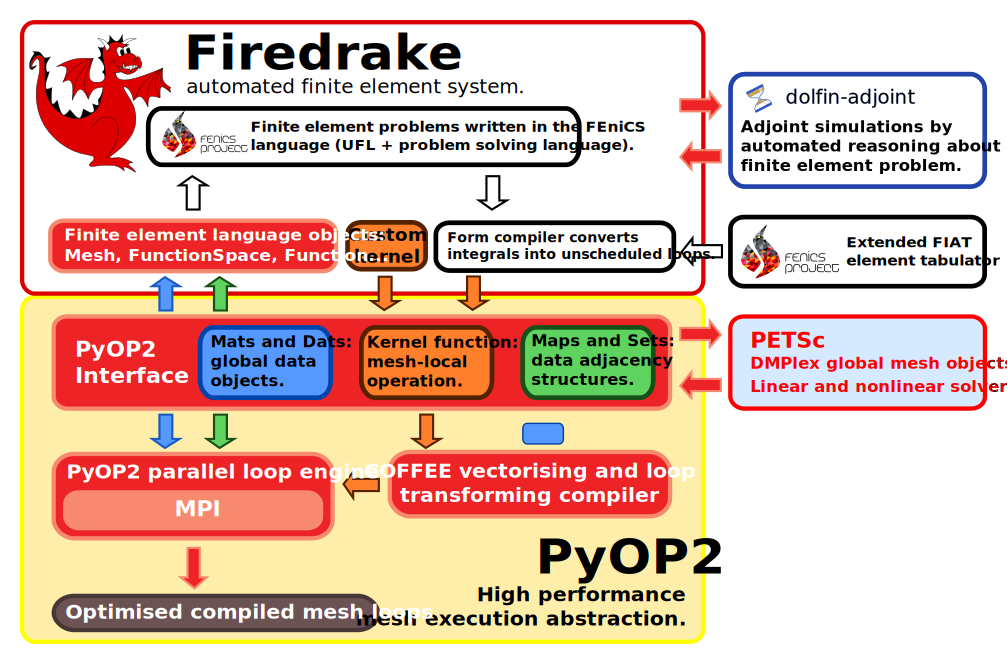
\includegraphics[width=\textwidth]{firedrake-stack}
\end{frame}

\section{Local kernels}

\begin{frame}
  \frametitle{Compiling variational forms}

  We use UFL \parencite{Alnaes:2014} from the FEniCS project for
  specifying variational problems.

  A \emph{form compiler} translates this to low-level executable code
  for evaluating the integral on an element.
\end{frame}

\begin{frame}[fragile]
  \frametitle{An example}
  \begin{columns}
    \begin{column}{0.5\textwidth}
\begin{minted}[fontsize=\tiny]{python}
mesh = UnitTriangleMesh()
V = FunctionSpace(mesh, "CG", 2)
u = TrialFunction(V)
v = TestFunction(V)
a = u*v*dx
\end{minted}
    \end{column}
\hspace{-3em}
    \begin{column}{0.65\textwidth}
\begin{minted}[fontsize=\tiny,mathescape]{c}
void integral(double A[6][6], 
    const double *restrict coords[6])
{
  double t0 = (-1 * coords[0][0]);
  double t1 = (-1 * coords[3][0]);
  /* $t2 \leftarrow |\det J|$ */
  double t2 = fabs(((t0 + (1 * coords[1][0])) *
                     (t1 + (1 * coords[5][0]))) +
                    (-1 * (t0 + (1 * coords[2][0])) *
                     (t1 + (1 * coords[4][0]))));
  static const double t3[6]     = {...};
  static const double t4[6][6]  = {...};
  for (int ip = 0; ip < 6; ip += 1) {
    double t5 = (t3[ip] * t2);
    for (int j = 0; j < 6; j += 1) {
      for (int k = 0; k < 6; k += 1) {
        A[j][k] += t5 * t4[ip][j] * t4[ip][k];
      }
    }
  }
}
\end{minted}
    \end{column}
  \end{columns}
\end{frame}
% \begin{frame}[fragile]
%   \frametitle{... and a complex one}
%   \begin{onlyenv}<1>
% \begin{minted}[fontsize=\tiny]{python}
% mesh = UnitTriangleMesh()
% V = VectorFunctionSpace(mesh, "CG", 2)
% P = VectorFunctionSpace(mesh, "CG", 2)
% v = TestFunction(V)
% du = TrialFunction(V)  # Incremental displacement
% u = Function(V)        # Displacement from previous iteration
% B = Function(V)        # Body force per unit mass
% # Kinematics
% I = Identity(v.cell().topological_dimension())
% F=I+grad(u)
% C = F.T*F
% E = (C - I)/2
% E = variable(E)
% # Material constants
% mu = Constant(1.0)
% lmbda = Constant(0.001)
% # Strain energy function (material model) 
% psi = lmbda/2*(tr(E)**2) + mu*tr(E*E)
% S = diff(psi, E)       # Second Piola-Kirchhoff stress tensor
% PK = F*S               # First Piola-Kirchoff stress tensor
% # Variational problem
% a = derivative((inner(PK, grad(v)) - inner(B, v))*dx, u, du)
% \end{minted}
%   \end{onlyenv}
%   \begin{onlyenv}<2>
% {\fontsize{3pt}{4pt}\selectfont
% \begin{columns}
% \begin{column}{0.5\textwidth}
% \begin{minted}{c}
% void integral(double A[12][12], const double *restrict coords[6],
%               const double *restrict w_0[12],
%               const double w_1[1],
%               const double w_2[1])
% {
%   double t0 = (-1 * coords[0][0]);
%   double t1 = (t0 + (1 * coords[1][0]));
%   double t2 = (-1 * coords[3][0]);
%   double t3 = (t2 + (1 * coords[5][0]));
%   double t4 = (t0 + (1 * coords[2][0]));
%   double t5 = (t2 + (1 * coords[4][0]));
%   double t6 = ((t1 * t3) + (-1 * t4 * t5));
%   double t7 = fabs(t6);
%   static const double t8[6]  = {...};
%   double t9 = (w_2[0] / 2);
%   double t10 = (1 * 1);
%   double t11 = (2 * t10);
%   double t12 = (-1 * 1);
%   double t13 = (t1 / t6);
%   double t14 = ((-1 * t4) / t6);
%   double t15 = ((-1 * t5) / t6);
%   double t16 = (t3 / t6);
%   static const double t17[6][12] = {...};
%   static const double  t18[6][12]  = {...};
%   static const double  t19[6][12]  = {...};
%   static const double  t20[6][12]  = {...};
%   for (int  ip  = 0; ip < 6; ip += 1) {
%     double  t59[12] ;
%     double  t60[12] ;
%     double  t65[12] ;
%     double  t66[12] ;
%     double  t24  = 0.0;
%     double  t23  = 0.0;
%     double  t22  = 0.0;
%     double  t21  = 0.0;
%     for (int  i_0  = 0; i_0 < 12; i_0 += 1) {
%       t21 += t20[ip][i_0] * w_0[i_0][0];
%       t22 += t19[ip][i_0] * w_0[i_0][0];
%       t23 += t18[ip][i_0] * w_0[i_0][0];
%       t24 += t17[ip][i_0] * w_0[i_0][0];
%     }
%     double  t25  = (1 + (t16 * t24) + (t15 * t23));
%     double  t26  = ((t14 * t24) + (t13 * t23));
%     double  t27  = ((t16 * t22) + (t15 * t21));
%     double  t28  = (1 + (t14 * t22) + (t13 * t21));
%     double  t29  = (t10 * (((t25 * t26) + (t27 * t28)) / 2));
%     double  t30  = ((t29 + t29) * w_1[0]);
%     double  t31  = ((t12 + (t25 * t25) + (t27 * t27)) / 2);
%     double  t32  = ((t12 + (t26 * t26) + (t28 * t28)) / 2);
%     double  t33  = (t11 * (t31 + t32) * t9);
%     double  t34  = (t10 * t31);
% \end{minted}
% \end{column}
% \begin{column}{0.5\textwidth}
% \begin{minted}{c}
%     double  t35  = (t33 + ((t34 + t34) * w_1[0]));
%     double  t36  = (t10 * t32);
%     double  t37  = (t33 + ((t36 + t36) * w_1[0]));
%     double  t38  = (t10 * (((t26 * t25) + (t28 * t27)) / 2));
%     double  t39  = ((t38 + t38) * w_1[0]);
%     for (int  k  = 0; k < 12; k += 1) {
%       double  t40  = ((t16 * t19[ip][k]) + (t15 * t20[ip][k]));
%       double  t41  = ((t14 * t17[ip][k]) + (t13 * t18[ip][k]));
%       double  t42  = (t41 * t25);
%       double  t43  = ((t16 * t17[ip][k]) + (t15 * t18[ip][k]));
%       double  t44  = (t43 * t26);
%       double  t45  = ((t14 * t19[ip][k]) + (t13 * t20[ip][k]));
%       double  t46  = (t45 * t27);
%       double  t47  = (t40 * t28);
%       double  t48  = (t10 * ((t42 + t44 + t46 + t47) / 2));
%       double  t49  = ((t48 + t48) * w_1[0]);
%       double  t50  = (t43 * t25);
%       double  t51  = (t40 * t27);
%       double  t52  = ((t50 + t50 + t51 + t51) / 2);
%       double  t53  = (t41 * t26);
%       double  t54  = (t45 * t28);
%       double  t55  = ((t53 + t53 + t54 + t54) / 2);
%       double  t56  = (t11 * (t52 + t55) * t9);
%       double  t57  = (t10 * t55);
%       double  t58  = (t56 + ((t57 + t57) * w_1[0]));
%       t59[k] = (t40 * t39) + (t49 * t27) + (t45 * t37) + (t58 * t28);
%       t60[k] = (t43 * t39) + (t49 * t25) + (t41 * t37) + (t58 * t26);
%       double  t61  = (t10 * t52);
%       double  t62  = (t56 + ((t61 + t61) * w_1[0]));
%       double  t63  = (t10 * ((t44 + t42 + t47 + t46) / 2));
%       double  t64  = ((t63 + t63) * w_1[0]);
%       t65[k] = (t40 * t35) + (t62 * t27) + (t45 * t30) + (t64 * t28);
%       t66[k] = (t43 * t35) + (t62 * t25) + (t41 * t30) + (t64 * t26);
%     }
%     double  t67  = (t8[ip] * t7);
%     for (int  j  = 0; j < 12; j += 1) {
%       double  t68  = ((t14 * t19[ip][j]) + (t13 * t20[ip][j]));
%       double  t69  = ((t14 * t17[ip][j]) + (t13 * t18[ip][j]));
%       double  t70  = ((t16 * t19[ip][j]) + (t15 * t20[ip][j]));
%       double  t71  = ((t16 * t17[ip][j]) + (t15 * t18[ip][j]));
%       for (int  k  = 0; k < 12; k += 1) {
%         A[j][k] += t67 * ((t66[k] * t71) + (t65[k] * t70) +
%                           (t60[k] * t69) + (t59[k] * t68));
%       }
%     }
%   }
% }
% \end{minted}
% \end{column}
% \end{columns}
% }
%   \end{onlyenv}
% \end{frame}

\begin{frame}
  \frametitle{Two-stage form compilation}
  \begin{enumerate}[<+->]
  \item Lower finite element expressions to tensor-algebra
  \item Lower tensor algebra to unscheduled loop nest of scalar
    expressions.
  \item Apply optimisation passes to minimise operation count, make
    code amenable to vectorising compilers.
  \end{enumerate}
  \uncover<+->{\centering
    \url{github.com/firedrakeproject/tsfc}
  }
\end{frame}
\begin{frame}
  \frametitle{Lowering FE}
  \begin{equation*}
    c_q = \sum_r \mathcal{E}_{q, r} c_r
  \end{equation*}
  $\mathcal{E}_{q, r}$ provided by FIAT as tabulation of 2D array.
  \begin{block}<2->{Structure in $\mathcal{E}$}
    \begin{equation*}
      \mathcal{E}_{q,r} = \mathcal{E}_{(q_x,r_x),(q_y, r_y)}
    \end{equation*}
    But $\mathcal{E}$ factorises
    \begin{equation*}
      \mathcal{E}_{q, r} = \mathcal{E}^x_{q_x, r_x}
      \mathcal{E}^y_{q_y, r_y}
    \end{equation*}
    WIP: exploiting structure for automated sum-factorisation.
  \end{block}
\end{frame}

\begin{frame}[fragile]
  \frametitle{Optimisation of finite element kernels}
  
  \begin{problem}<+->
    Modern optimising compilers do a bad job on finite element
    kernels.
  \end{problem}
  \begin{exampleblock}<+->{Code motion (or not?)}
\begin{minted}[fontsize=\scriptsize]{c}
for (i = 0; i < L; i++ )
   for (j = 0; j < M; j++)
      for (k = 0; k < N; k++)
         A[j][k] += f(i, j)*g(i, k)
\end{minted}
  \end{exampleblock}
  \begin{corollary}<+->
    We need to spoon-feed the compiler already optimised code.
  \end{corollary}
\end{frame}
\begin{frame}[allowframebreaks]
  \frametitle{COFFEE}

  No single optimal schedule for evaluation of every finite element
  kernel.  Variability in
  \begin{itemize}
  \item polynomial degree,
  \item number of fields,
  \item kernel complexity,
  \item working set size,
  \item structure in the basis functions,
  \item structure in the quadrature points,
  \item ...
  \end{itemize}
  We \emph{explore} (some of) this space using a special-purpose
  compiler.

\pagebreak

\begin{block}{Flop reduction}
  Exploit \emph{linearity} in test functions to perform factorisation,
  code motion and CSE.  

Cost model: don't introduce mesh-sized
  temporaries.\\
  \cite{Luporini:2016} \arxivlink{1604.05872}{cs.MS}
\end{block}

\begin{block}{Vectorisation}
  Align and pad data structures, then use intrinsics or rely on
  compiler.  Experience, gcc-4.X \emph{really} doesn't want to
  vectorise short loops!\\
  \cite{Luporini:2015} \doilink{10.1145/2687415}
\end{block}
\begin{center}
  \url{github.com/coneoproject/COFFEE}
\end{center}
\end{frame}

\section{Global iteration}

\begin{frame}[fragile]
  \frametitle{PyOP2}
  A library for expressing data parallel iterations
\begin{description}
\item[{\emph{Sets}}] iterable entities
\item[{\emph{Dats}}] abstract managed arrays (data defined on a set)
\item[{\emph{Maps}}] relationships between elements of sets
\item[{\emph{Kernels}}] local computation
\item[{\emph{par\_loop}}] Data parallel iteration over a set
\end{description}
Arguments to parallel loop indicate how to gather/scatter global
data using \emph{access descriptors}

\begin{minted}[fontsize=\scriptsize]{python}
par_loop(kernel, iterset, data1(map1, READ), data2(map2, WRITE))
\end{minted}
\end{frame}

\begin{frame}
  \frametitle{Key ideas}
  \begin{block}{Local computation}
    Kernels do not know about global data layout.
    \begin{itemize}
    \item Kernel defines contract on local, packed, ordering.
    \item Global-to-local reordering/packing appears in map.
    \end{itemize}
  \end{block}
  \begin{block}{``Implicit'' iteration}
    Application code does not specify explicit iteration order.
    \begin{itemize}
    \item Define data structures, then just ``iterate''
    \item Can't write Gauss-Seidel (for example)
    \item Lazy evaluation
    \end{itemize}
  \end{block}
\end{frame}

\begin{frame}[allowframebreaks]
  \frametitle{Tensions in model development}

  \begin{block}{Performance}
    \begin{itemize}
    \item Keep data in cache as long as possible.  
    \item Manually fuse kernels.
    \item Loop tiling for latency hiding.
    \item ...
    \item Individual components hard to test
    \item Space of optimisations suffers from combinatorial
      explosion.
    \end{itemize}
  \end{block}

\pagebreak
  \begin{block}{Maintainability}
    \begin{itemize}
    \item Keep kernels separate
    \item ``Straight-line'' code
    \item ...
    \item Testable
    \item Performance of individual kernels may be good, but can throw
      away \emph{a lot}
    \end{itemize}
  \end{block}

\end{frame}
\begin{frame}
  \begin{exampleblock}{Lazy evaluation}
    \begin{itemize}
    \item \verb~par\_loop~ only executed ``when you look at the
      data''.
    \item PyOP2 sees sequence of loops, can reason about them for
      \begin{itemize}
      \item Loop fusion
      \item Loop tiling
      \item Communication coalescing
      \end{itemize}
    \end{itemize}
  \end{exampleblock}

  Application code does not change.  ``What, not how''.
\end{frame}

\begin{frame}[fragile]
  \frametitle{Another example: extruded meshes}
  In many geophysical applications, meshes are topologically \emph{structured} in
  the (short) vertical direction.

  Can produce vertically structured dof-numbering, avoiding most of
  the indirection penalty.

  Only need to annotate data structures with this extra information.
\begin{minted}[fontsize=\tiny]{python}
s = Set(100) # Unstructured set
e = ExtrudedSet(s, layers=...) # Semi-structured set
d = DataSet(...)
# values encode indirections on base set
# offsets say how to move in the structured direction
map = Map(e, d, values, offsets=[...])

par_loop(kernel, e, data(map, WRITE), ...)
\end{minted}
\end{frame}

\begin{frame}
  \begin{center}
    \includegraphics[height=0.8\textheight]{extruded-performance}

    \cite{Bercea:2016} \arxivlink{1604.05937}{cs.MS}
  \end{center}
\end{frame}


\section{Did we succeed?}

\begin{frame}
  \frametitle{Experimentation}
  
  With model set up, experimentation is easy

  \begin{itemize}
  \item Change preconditioner: c. 1 line
  \item Drop terms: c. 1-4 lines
  \item Different operator: c. 1-10 lines
  \item quasi-Newton: c. 1-10 lines
  \item Matrix-free: XXX
  \end{itemize}
\end{frame}

\begin{frame}
  \frametitle{Maintainability}
  \begin{columns}
    \begin{column}[t]{0.5\textwidth}
      \begin{block}{Core Firedrake}
        \begin{table}
          \centering
          \begin{tabular}{lc}
            Component & LOC \\
            \hline
            Firedrake & 9000 \\
            PyOP2     & 5000 \\
            TSFC      & 2700 \\
            COFFEE    & 4500 \\
            \hline
            Total     & 21200
          \end{tabular}
        \end{table}
      \end{block}
    \end{column}
    \begin{column}[t]{0.5\textwidth}
      \begin{block}{Shared with FEniCS}
        \begin{table}
          \centering
          \begin{tabular}{lc}
            Component & LOC \\
            \hline
            FIAT & 4000 \\
            UFL     & 13000 \\
            \hline
            Total & 17000
          \end{tabular}
        \end{table}        
      \end{block}
    \end{column}
  \end{columns}
\end{frame}
\begin{frame}[allowframebreaks]
  \frametitle{Performance}

  \begin{block}{Multigrid for NWP}
    \begin{itemize}
    \item Horizontal coarsening with vertical line relaxation to treat
      strong anisotropy.
    \item UFL used for operators, plus custom PyOP2 kernels for banded
      matrix algebra
    \item Bandwidth limited, achieve $> 55\%$ STREAM triad.
    \item \cite{Mitchell:2016} \arxivlink{1605.00492}{cs.MS}
    \end{itemize}
  \end{block}

\pagebreak

  \begin{columns}
    \begin{column}{0.7\textwidth}
      \begin{block}{Thetis}
        \begin{itemize}
        \item 3D unstructured coastal ocean model in Firedrake
        \item Lock exchange test case
          \begin{description}
          \item[Thetis] P1DG-P1DG, triangular wedges.  $13s/s$.
          \item[SLIM] hand-coded/optimised (same discretisation),
            $6s/s$
          \end{description}
        \end{itemize}
      \end{block}
    \end{column}
    \begin{column}[t]{0.3\textwidth}
      \includegraphics[width=2.5cm]{thetis_logo}
    \end{column}
  \end{columns}
  \begin{center}
    \url{github.com/thetisproject/thetis}    
  \end{center}
\end{frame}

\begin{frame}[fragile]
  \frametitle{Abstraction degradation}
  Exposing PyOP2 provides means of writing mesh iterations that are
  not ``assemble a variational form''.

  \begin{exampleblock}{Slope limiters}
    Vertex-based limiters need max/min over incident cells
\begin{minted}[fontsize=\tiny]{python}
par_loop("""
    for (int i=0; i<qmax.dofs; i++) {
        qmax[i][0] = fmax(qmax[i][0], centroids[0][0]);
        qmin[i][0] = fmin(qmin[i][0], centroids[0][0]);
    }
    """,
       dx,
       {'qmax': (max_field, RW),
        'qmin': (min_field, RW),
        'centroids': (centroids, READ)})
\end{minted}
  \end{exampleblock}
\end{frame}

\begin{frame}
  \frametitle{Coming (soon)}
  \begin{itemize}
  \item Efficient high order evaluation (via tensor-products and/or
    Bernstein polynomials)
  \item Matrix-free operators and preconditioning
  \item Symbolic (not just algebraic) composition for multiphysics
    preconditioning
  \item Mesh adaptivity
  \item ...
  \end{itemize}
\end{frame}

\begin{frame}[standout]
  Questions?
\end{frame}

\appendix
\begin{frame}[allowframebreaks]
  \frametitle{References}
  \printbibliography[heading=none]
\end{frame}
\end{document}
